\documentclass[11pt,fleqn]{article} % Default font size and left-justified equations

%\usepackage{standalone}

\usepackage{todonotes}
\usepackage{color}
% use \todo{note} OR \missingfigure{Add my picture here}

\usepackage[top=3cm,bottom=3cm,left=3.2cm,right=3.2cm,headsep=10pt,a4paper]{geometry} % Page margins
\usepackage{xcolor} % Required for specifying colors by name
\definecolor{ocre}{RGB}{243,102,25} % Define the orange color used for highlighting throughout the book


% Font Settings


% SLG commented out


% \usepackage{avant} % Use the Avantgarde font for headings
%\usepackage{times} % Use the Times font for headings
% \usepackage{microtype} %Slightly tweak font spacing for aesthetics
% \usepackage{mathptmx} % Use the Adobe Times Roman as the default text font together with math symbols from the Sym­bol, Chancery and Com­puter Modern fonts


%  \usepackage[scaled=0.90]{couriers} %What is this used for?




% SLG commented out
% \def\thereforesymbol{
% \leavevmode
% \lower0.1ex\hbox{$\cdot$}
% \kern-0.2em\raise0.7ex\hbox{$\cdot$}
% \kern-0.2em\lower0.2ex\hbox{$\cdot$}
% \thinspace}


% \usepackage{CJKutf8}
%For cyrillic characters  (do we have any?)


% slg commented this out:
% \usepackage[OT2,T1]{fontenc}
% \DeclareSymbolFont{cyrletters}{OT2}{wncyr}{m}{n}
% \DeclareMathSymbol{\Sha}{\mathalpha}{cyrletters}{"58}


\usepackage[T1]{fontenc}
\usepackage[section]{placeins}

% slg commented these out:
% \usepackage{amssymb}
 \usepackage{fancyvrb}
%  \usepackage{color}




%define a verbatim text for bold user input
\newcommand\verbbf[1]{\textbf{$\blacksquare$ #1}}
%define a verbatim text without box in front
\newcommand\verbbnbf{\textbf}


\PassOptionsToPackage{hyphens}{url}


\usepackage[pdftitle={Users Manual for the hashdb toolset},
              pdfauthor={Bruce Allen, Jessica R. Bradley, Simson L. Garfinkel},
              pdfkeywords={hashdb, block hash database}]{hyperref}
\makeatletter
\g@addto@macro{\UrlBreaks}{\UrlOrds}
\makeatother
% \usepackage{microtype} % Slightly tweak font spacing for aesthetics
%\usepackage[utf8]{inputenc} % Required for including letters with accents
\usepackage[T1]{fontenc} % Use 8-bit encoding that has 256 glyphs




%\usepackage[a4paper,pdftex]{geometry}                                                                                % A4paper margins
\setlength{\oddsidemargin}{5mm}                                                                                                % Remove 'twosided' indentation
\setlength{\evensidemargin}{5mm}


\usepackage[english]{babel}
%\usepackage[protrusion=true,expansion=true]{microtype}        
\usepackage{amsmath,amsfonts,amsthm,amssymb}
\usepackage{graphicx}


\usepackage{tabularx}


% Simson commented this out:
%use autoref or Autoref for lowercase or uppercase beginning of references
\usepackage{catoptions}
\makeatletter
\def\figureautorefname{figure}
\def\tableautorefname{table}
\def\Autoref#1{%
  \begingroup
  \edef\reserved@a{\cpttrimspaces{#1}}%
  \ifcsndefTF{r@#1}{%
    \xaftercsname{\expandafter\testreftype\@fourthoffive}
      {r@\reserved@a}.\\{#1}%
  }{%
    \ref{#1}%
  }%
  \endgroup
}
\def\testreftype#1.#2\\#3{%
  \ifcsndefTF{#1autorefname}{%
    \def\reserved@a##1##2\@nil{%
      \uppercase{\def\ref@name{##1}}%
      \csn@edef{#1autorefname}{\ref@name##2}%
      \autoref{#3}%
    }%
    \reserved@a#1\@nil
  }{%
    \autoref{#3}%
  }%
}
\makeatother


\usepackage{amsmath}


\usepackage{booktabs}


% slg commented out:
% \usepackage{makecell}


\usepackage{color}
\usepackage{graphicx}
%\usepackage {hyperref}
\usepackage{listings}
\usepackage{xspace}


% slg commented out:
\usepackage[toc, page]{appendix}
\usepackage[labelfont=bf]{caption}
%http://tex.stackexchange.com/questions/27663/using- bold-italic-text-inside-listings


% slg commented out:
% \usepackage{multirow} %for multirow tables




\newcommand{\HRule}{\rule{\linewidth}{0.5mm}}
\usepackage{fancyhdr}


\usepackage{array}



\setcounter{secnumdepth}{5}
\setcounter{tocdepth}{5}
 
%\usepackage{arabtex}

\usepackage{verbatim}

\raggedbottom

\begin{document}

%define macros for commonly used terms that require special formatting
\newcommand \hash {\textit{hashdb}\xspace}
\newcommand \bulk {\textbf{bulk\_extractor}\xspace}

\hypersetup{%
    pdfborder = {0 0 0}
}

\lstdefinestyle{customfile}{
basicstyle=\footnotesize\ttfamily, frame=single, float=htpb}

\begin{titlepage}





% LaTeX Template: Titlepage
% This is a title page template which be used for both articles and reports.
%
% Copyright: http://www.howtotex.com/
% Date: April 2011
% ------------------------------------------------------------------------------

% -------------------------------------------------------------------------------
% Preamble
% -------------------------------------------------------------------------------
%\documentclass[paper=a4, fontsize=11pt,twoside]{scrartcl}		% KOMA article


% ------------------------------------------------------------------------------
% Definitions (do not change this)
% ------------------------------------------------------------------------------
\newcommand{\TRule}[1]{\rule{\linewidth}{#1}} 	% Horizontal rule

\makeatletter							% Title
\def\printtitle{%						
    {\centering \@title\par}}
\makeatother									

\makeatletter							% Author
\def\printauthor{%					
    {\centering \large \@author}}				
\makeatother							

% ------------------------------------------------------------------------------
% Metadata (Change this)
% ------------------------------------------------------------------------------
\title{	\LARGE \textsc{\textit{hashdb 3.1.0}} 	% Subtitle of the document
		 	\\[1.0cm]													% 2cm spacing
			\TRule{0.5pt} \\										% Upper rule
			\LARGE \textbf{\uppercase{Users Manual}}	% Title
			\TRule{2pt} \\ [0.5cm]								% Lower rule + 0.5cm spacing
			\normalsize \today									% Todays date
		}
\author{
		Authored by: \\
		Bruce D. Allen\\
		Jessica R. Bradley\\
		Simson L. Garfinkel\\		
}

% ------------------------------------------------------------------------------
% Maketitle
% ------------------------------------------------------------------------------
\thispagestyle{empty}				% Remove page numbering on this page

\printtitle									% Print the title data as defined above
  	\vfill
\printauthor								% Print the author data as defined above














\end{titlepage}


\pagenumbering{roman}
\setlength{\parindent}{0pt} %remove indenting from whole document
\newpage
\thispagestyle{empty}
\mbox{}
\newpage
\section*{One Page Quickstart for Linux and Mac Users}
This page provides a very brief introduction to downloading, installing and running \hash (creating a database and populating it) on Linux and MacOS systems. 
\begin{enumerate}
\item Download the latest version of \hash. It can be obtained from \url{http://digitalcorpora.org/downloads/hashdb}. The file is called \texttt{hashdb-x.y.z.tar.gz} where x.y.z is the latest version. 

\item Un-tar and un-zip the file.  In the newly created \textit{hashdb-x.y.z} directory, run the following commands:

\begin{Verbatim}[commandchars=\\\{\}]
\verbbf{./configure}
\verbbf{make}
\verbbf{sudo make install}
\end{Verbatim}
[Refer to \textbf{\Autoref{Installation}}. Note, for full functionality, some users may need to first download and install dependent library files. Instructions are outlined in the referenced section.]

\item Navigate to the directory where you would like to create a hash database. Then, to run \hash from the command line, type the following instructions: 
\begin{Verbatim}[commandchars=\\\{\}]
\verbbf{hashdb create sample.hdb}
\end{Verbatim} 

In the above instructions, \textit{\textbf{sample.hdb}} is that empty database that will be created with default database settings. 

\item Next, import data into the database, you will need a DFXML file containing block hash values. If you do not already have one, see \textbf{\Autoref{createDFXML}} for instructions on creating one. To populate the hash database with the hashes from the DFXML file called \texttt{sample.xml}, type the following instructions from the directory where you created the database:
\begin{Verbatim}[commandchars=\\\{\}]
\verbbf{hashdb import sample.xml sample.hdb}
\end{Verbatim} 
This command, if executed successfully, will print the number of hash values inserted. For example: 
\begingroup
\footnotesize
\begin{Verbatim}[fontfamily=courier]
hashdb changes (insert):
    hashes inserted: 2595
\end{Verbatim}
\endgroup
\item Additionally, the file \texttt{log.xml} contained in the directory \textit{sample.hdb} will be updated with change statistics. It will show the number of hash values that have been inserted [see \textbf{\Autoref{updateSection} }for more information on the change statistics tracked in the log file].
\end{enumerate}
\newpage

\section*{One Page Quickstart for Windows Users}
 This page provides a very brief introduction to downloading, installing and running \hash on Windows systems. 
\begin{enumerate}
\item Download the windows installer for the latest version of \hash. It can be obtained from \url{http://digitalcorpora.org/downloaads/hashdb}. The file is called \texttt{hashdb-x.y.z-windowsinstaller.exe} where x.y.z is the latest version. 

\item Run the installer file. This will automatically install \hash on your machine.

\item Navigate to the directory where you would like to create a hash database. Then, to run \hash from the command line, type the following instructions: 
\begin{Verbatim}[commandchars=\\\{\}]
\verbbf{hashdb create sample.hdb}
\end{Verbatim} 

In the above instructions, \textit{\textbf{sample.hdb}} is that empty database that will be created with default database settings.

\item Next, import data into the database, you will need a DFXML file containing sector hash values. If you do not already have one, see \textbf{\Autoref{createDFXML}} for instructions on creating one. To populate the hash database with the hashes from the DFXML file called \texttt{sample.xml}, type the following instructions from the directory where you created the database:
\begin{Verbatim}[commandchars=\\\{\}]
\verbbf{hashdb import sample.xml sample.hdb}
\end{Verbatim} 
This command, if executed successfully, will print the number of hash values inserted. For example: 
\begingroup
\footnotesize
\begin{Verbatim}[fontfamily=courier]
hashdb changes (insert):
    hashes inserted: 2595
\end{Verbatim}
\endgroup
\item Additionally, the file \texttt{log.xml} contained in the directory \textit{sample.hdb} will be updated with change statistics. It will show the number of hash values that have been inserted [see \textbf{\Autoref{updateSection}} for more information on the change statistics tracked in the log file].
 

\end{enumerate}

\newpage


\tableofcontents
\newpage
\pagenumbering{arabic}





\newpage

\section{Introduction}
\subsection {Overview of \hash}
\hash is a tool that can be used to find data in raw media using cryptographic hashes calculated from blocks of data. It is a useful forensic investigation tool for tasks such as malware detection, child exploitation detection or corporate espionage investigations. The tool provides several capabilities that include:
\begin{itemize}
\item Creating hash databases of MD5 block hashes, as opposed to file hashes.
\item Importing hash values from Digital Forensic XML (DFXML) files created by other programs such as \textbf{md5deep}.
\item Scanning the hash database for matching hash values using either the local or remote system. 
\item Providing the source information for hash values. 
\end{itemize}

Using \hash, a forensic investigator can take a known set of blacklisted media and generate a hash database. The investigator can then use the hash database to search against raw media for blacklisted information. For example, given a known set of malware, an investigator can generate a sector hash database representing that malware. The investigator can then search a given corpus for fragments of that malware and identify the specific malware content in the corpus using \hash and the \bulk program. \\

\hash relies on block hashing rather than full file hashing. Block hashing provides an alternative methodology to file hashing with a different capability set. With file hashing, the file must be complete to generate a file hash, although a file carver can be used to pull together a file and generate a valid hash.  File hashing also requires the ability to extract files, which requires being able to understand the file system used on a particular storage device. Block hashing, as an alternative, does not need a file system or files. Artifacts are identified at the block scale (usually 4096 bytes) rather than at the file scale. While block hashing does not rely on the file system, artifacts do need to be sector-aligned for \hash to find hashes \cite{hashEncoding}.\\

\hash provides an advantage when working with hard disks and operating systems that fragment data into discontiguous blocks yet still sector-align media. This is because scans are performed along sector boundaries. Because \hash works at the block resolution, it can find part of a file when the rest of the file is missing, such as with a large video file where only part of the video is on disk. \hash can also be used to analyze network traffic (such as that captured by \textbf{tcpflow}).  Finally, \hash can identify artifacts that are sub-file, such as embedded content in a \texttt{.pdf} document.\\

\hash stores cryptographic hashes (along with their source information) that have been calculated from hash blocks. It also provides the capability to scan other media for hash matches. Many of the capabilities of \hash are best utilized in connection with the \bulk program. This manual describes uses cases for the \hash tools, including its uses with \bulk and demonstrates how users can take full advantage of all of its capabilities.

\subsection{Purpose of this Manual}
This Users Manual is intended to be useful to new, intermediate and experienced users of \hash. It provides an in-depth review of the functionality included in \hash and shows how to access and utilize features through command line operation of the tool. This manual includes working examples with links to the input data used, giving users the opportunity to work through the examples and utilize all aspects of the system. 

\subsection{Conventions Used in this Manual}
This manual uses standard formatting conventions to highlight file names, directory names and example commands. The conventions for those specific types are described in this section. \\

Names of programs including the post-processing tools native to \hash and third-party tools are shown in \textbf{bold}, as in \textbf{bulk\_extractor}.\\

File names are displayed in a fixed width font. They will appear as \texttt{filename.txt} within the text throughout the manual.\\

Directory names are displayed in italics. They appear as \textit{directoryname/} within the text. The only exception is for directory names that are part of an example command. Directory names referenced in example commands appear in the example command format.\\

Database names are denoted with bold, italicized text. They are always specified in lower-case, because that is how they are referred in the options and usage information for \hash. Names will appear as \textbf{\textit{databasename}}.\\

This manual contains example commands that should be typed in by the user. A command entered at the terminal is shown like this: \begin{Verbatim}[commandchars=\\\{\}]
\verbbf{command}
\end{Verbatim}

The first character on the line is the terminal prompt, and should not be typed. The black square is used as the standard prompt in this manual, although the prompt shown on a users screen will vary according to the system they are using.\\


\section{How \hash Works}
The \hash tool provides capabilities to create, edit, access and search databases of cryptographic hashes created from hash blocks. The cryptographic hashes are imported into a database from DFXML files created by other programs (which could include \textbf{md5deep}) or exported from another \hash database. \hash databases can also be populated using \bulk and the \textit{hashdb} scanner. Once a databases is created, \hash provides users with the capability to scan the database for matching hash values and identify matching content. Hash databases can also be exported, added to, subtracted from and shared.\\


Figure \ref{fig:overviewFigure} provides an overview of the capabilities included with the \hash tool. \hash populates databases from DFXML files created by other programs. The sources of those files can be virtually any type of raw digital media including black list files and disk images. Users can also add or remove data from the database after it is created. Once the database is populated, \hash can export content from the database in DFXML format. It also provides an API that can be used by third party tools (as it is used in the \bulk program) to create, populate and access hash databases. Finally, \hash allows users to scan the hash database for matching hash values.\\
\begin{figure}
	\center
	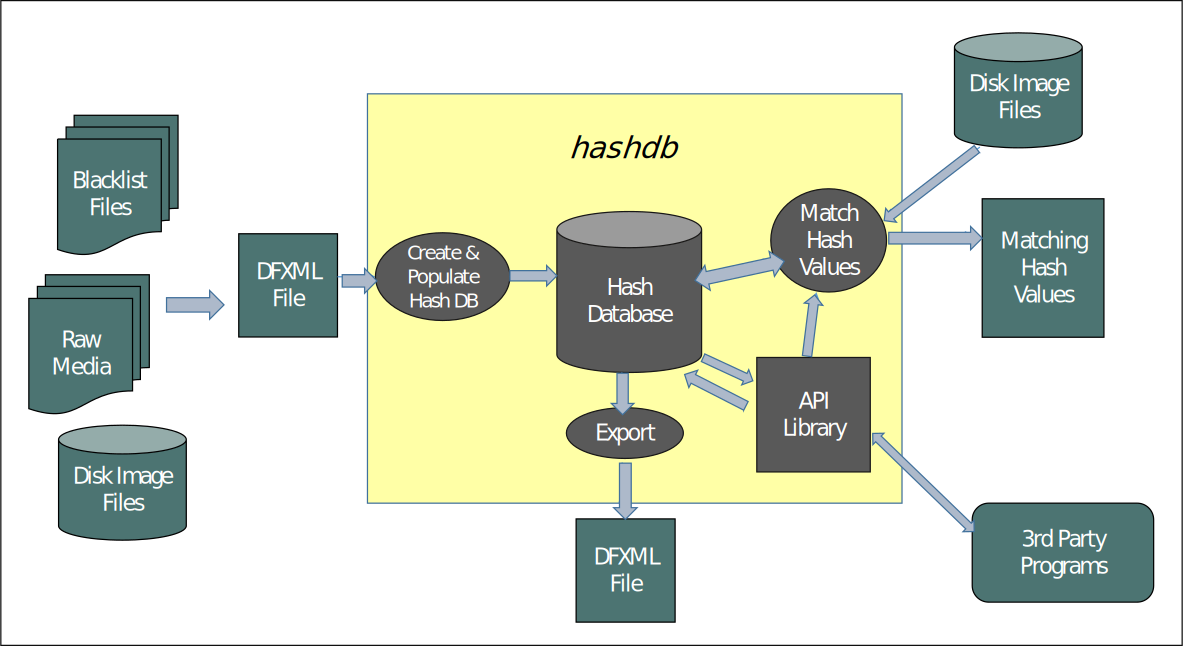
\includegraphics[scale=.45]{drawings/hashdb_system_overview}
	\caption{Overview of the \hash system}
	\label{fig:overviewFigure}
\end{figure}

\subsection{Hash Blocks}
\hash relies on block hashing rather than file hashing. A hash block is a contiguous sequence of bytes, typically 4KiB in size. Tools using block hashing calculate cryptographic hashes from hash blocks, along with information about where the hash blocks are sourced from. To increase the probability of finding matching hashes in sector-based disk images, hashes are generated at each sector boundary. Figure \ref{fig:sectorboundaries} illustrates cryptographic hashes generated from 4KiB hash blocks aligned on 512 byte sector boundaries. Block size is selectable in tools such as \textbf{md5deep}. In our work, we use a block size of 4KiB.\\

\begin{figure}
	\center
	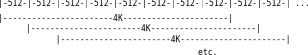
\includegraphics[scale=1.1]{drawings/sector_boundaries}
	\caption{Hashes generated over overlapping sector boundaries. 4K lines represent the hash blocks.}
	\label{fig:sectorboundaries}
\end{figure}



\subsection{DFXML}
\hash populates the hash databases using DFXML files (or via the API using the import command, introduced in Section \ref{usingSection}). DFXML is an XML language designed to represent a wide range of forensic information and forensic processing results. It allows the sharing of structured information between independent tools and organizations \cite{dfxmlpaper}.\\

The \textbf{md5deep} tool creates cryptographic hashes from hash blocks and produces DFXML files. Listing \ref{md5excerpt} shows an excerpt of the DFXML file created by \textbf{md5deep}. The portion of the file of interest to \hash is contained in the ``byte\_run'' tag. The ``file\_offset'' attribute is the number of bytes into the file where the cryptographic block hash was calculated. The The  ``len'' attribute indicates the size of the block.  The ``hashdigest'' tag identifies that hash algorithm (MD5) and the long hexadecimal hash value. The ``filename'' tag indicates the filename to which the hashes can be attributed. \\
\lstset{style=customfile}
\begin{lstlisting}[float, caption=Excerpt of a DFXML report file showing the MD5 output, label=md5excerpt]
  <fileobject>
    <filename>/home/bdallen/demo/mock_video.mp4</filename>
    <filesize>10630146</filesize>
    <ctime>2014-01-30T20:20:39Z</ctime>
    <mtime>2014-01-30T19:04:59Z</mtime>
    <atime>2014-01-30T20:04:52Z</atime>
    <byte_run file_offset='0' len='4096'>   
      <hashdigest type='MD5'>63641a3c008a3d26a192c778dd088868</hashdigest>
    </byte_run>
    <byte_run file_offset='4096' len='4096'>   
      <hashdigest type='MD5'>c7dd2354e223c10856469e27686b8c6b</hashdigest>
    </byte_run>
    <byte_run file_offset='8192' len='4096'>   
      <hashdigest type='MD5'>ff540fda05d008ccebf2cca2ec71571d</hashdigest>
    </byte_run>
    <byte_run file_offset='12288' len='4096'>   
      <hashdigest type='MD5'>d3de47d704e85e0f61a91876236593d3</hashdigest>

...

    <byte_run file_offset='10625024' len='4096'>   
      <hashdigest type='MD5'>d2d958b44c481cc41b0121b3b4afae85</hashdigest>
    </byte_run>
    <byte_run file_offset='10629120' len='1026'>   
      <hashdigest type='MD5'>4640564a8655d3b201a85b4a76411b00</hashdigest>
    </byte_run>
    <hashdigest type='MD5'>a003483521c181d26e66dc09740e939d</hashdigest>
  </fileobject>

\end{lstlisting}  

\subsubsection{Creating a DFXML file}
\label{createDFXML}
Users may create DFXML files to import hashes from by using the
\textbf{md5deep} tool.
\textbf{md5deep} is available at \url{http://md5deep.sourceforge.net}.
For additional instructions on downloading and installing
\textbf{md5deep}, go to \url{http://github.com/simsong/hashdb/wiki/Installing-md5deep}.\\

Choose a file or directory to use as the source of data for the hash file output. For this manual, we use the file \texttt{mock\_video.mp4} available at \url{http://digitalcorpora.org/downloads/hashdb/demo/}. Then, run \textbf{md5deep} with the following command:\\
\begin{Verbatim}[commandchars=\\\{\}]
\verbbf{md5deep -p 4096 -d mock_video.mp4 > mock_video.xml}
\end{Verbatim}
The above command specifies:
\begin{itemize}
\item a block size of 4096 bytes (\textbf{-p} option) 
\item that the hash output will be written to a DFXML file (\textbf{-d} option)
\item to write the output to the file \texttt{mock\_video.xml}. The  $>$ symbol specification writes the output into the file 
\end{itemize}
 The file \texttt{mock\_video.xml} will be used in the next step to create the hash database. However, any DFXML file containing block hash values can be used in \hash.\\

Note, for this example we are using only one file to populate the DFXML. However, users will typically be creating a block hash file from thousands of files in hundred of directories. To create a block hash file that recursively includes all files and directories contained within a directory, use the command \textbf{mdf5deep -r $<$directoryname$>$} along with the other options specified above.

\subsection{Contents of a Hash Database}
Each \hash database is contained in a directory called \textit{$<$databasename$>$.hdb} and contains a number of files. These files are:
\begin{verbatim}
Bloom_filter_1
hash_store
history.xml
log.xml
settings.xml
source_filename_store.dat
source_filename_store.idx1
source_filename_store.idx2
source_lookup_store.dat
source_lookup_store.idx1
source_lookup_store.idx2
source_repository_name_store.dat
source_repository_name_store.idx1
source_repository_name_store.idx2
\end{verbatim}

These files include XML files containing configuration settings and logs, a Bloom filter file used for improving the speed of hash lookups, binary files containing stored hashes from multiple sources and binary files that allow lookup of hash source names. Of these files, the following may be of interest to the user:
\begin{itemize}
\item \texttt{log.xml} \\
Every time a command is run that changes the content of the database, this file is replaced with a log of the run.
The log includes the command name, information about \hash including the command typed and how \hash was compiled, information about the operating system \hash was just run on, a copy of the \hash settings, timestamps indicating how much time the command took, and the specific \hash changes applied, described in more detail in Section \ref{updateSection}.
\item \texttt{settings.xml} \\
This file includes the build environment and execution environment, described above, and the settings requested by the user when the block hash database was created, see \hash settings and Bloom filter settings options.
\item \texttt{history.xml} \\
The purpose of this file is to retain full attribution for a database.
On every change, \texttt{log.xml} is appended.
On every change applied from another database
(or from two databases, as is the case with the \texttt{add\_multiple} command),
the history of that database or databases is also appended.
It can be difficult to follow for all but advanced users but provides full attribution nonetheless.
\end{itemize}



\subsection{Using the Hash Databases}
\label{usingSection}
\hash provides the capability for users to scan the database for matching hash blocks locally or remotely via a socket. Users can also query for hash source information and information about the hash database itself. \hash provides an API to access the import and scan capabilities.  The import capability allows third party tools to create a new database at a specified directory, import an array of hashes with source information and write changes to the \texttt{log.xml} file. The scan capability provided by the API allows third party tools to open an existing database and perform a scan. Most importantly, the \bulk \textit{hashdb} scanner uses the \hash API to provide users with the capability to create databases from disk images or scan digital media and find matching hash blocks within the data \bulk is processing. In later sections, this manual describes the methods for using \bulk together with the \hash tool. 

\subsubsection{\bulk}
\bulk is an open source digital forensics tool that extracts features such as email addresses, credit card numbers, URLs and other types of information from digital evidence files. It operates on disk images, files or a directory of files and extracts useful information without parsing the file system or file system structures.  For more information on how to use \bulk for a wide variety of applications, refer to the separate publication \textit{The \bulk Users Manual} available at \url{http://digitalcorpora.org/downloads/bulk_extractor/BEUsersManual.pdf} \cite{beusersguide}.\\

\bulk has multiple scanners that extract features. One particular scanner, the \textit{hashdb} scanner links the full set of \bulk capabilities directly to the \hash tool. The \textit{hashdb} scanner uses the \hash API to create and import data into hash databases  directly from the data processed by \bulk. The scanner also can be run with a hash database as input (again using the \hash API) will scan the data processed by \bulk for matching hash values.\\

The functionality of \hash is provided through command line operation and the available API. The following section describes how to download, install and run \hash. 
\section{Running \hash}
\hash is a command line tool that can be run on Linux, MacOS or Windows systems. Here we describe the installation procedures for those system as well as the basic commands used to run the tool, including creating and maintaining a database and scanning media for hash values.

\subsection{Installation Guide}
The following sections explain how to install the required dependencies as well as download \hash and compile the release or run the executable. 
\label{Installation}

\subsubsection{Installing on Linux or Mac}

Before compiling \hash for your platform, you may need to install other packages on your system which \hash requires to compile cleanly and with a full set of capabilities.\\

\textbf{Dependencies for Linux}\\
The following commands should add the appropriate packages:
\begin{Verbatim}[commandchars=\\\{\}]
\verbbf{sudo yum update}
\verbbf{sudo yum groupinstall development-tools}
\verbbf{sudo yum install gcc-c++}
\verbbf{sudo yum install libxml2-devel openssl-devel tre-devel boost-devel}
\end{Verbatim}

\textbf{Dependencies for Mac Systems}\\
Mac users must first install Apple's Xcode development system. Other components should be downloaded using the MacPorts system. If you do not have MacPorts, go to the App store and download and install it. It is free. Once it is installed, try:
\begin{Verbatim}[commandchars=\\\{\}]
\verbbf{sudo port install autoconf automake libxml2} 
\end{Verbatim}

\textbf{Download and Install \hash}\\
Next, download the latest version of \hash. The software can be downloaded from \url{http://digitalcorpora.org/downloads/hashdb/}. The file to download is \texttt{hashdb-x.y.z.tar.gz} where x.y.z is the latest version. As of publication of this manual, the latest version of \hash is 1.0.0.\\


After downloading the file, un-tar it by either right-clicking on the file and choosing ``extract to...' or typing the following at the command line:
\begin{Verbatim}[commandchars=\\\{\}]
\verbbf{tar -xvf hashdb-x.y.z.tar.gz}
\end{Verbatim}

Then, in the newly created \textit{hashdb-x.y.z} directory, run the following commands to install \hash in \textit{/usr/local/bin} (by default):

\begin{Verbatim}[commandchars=\\\{\}]
\verbbf{./configure}
\verbbf{make}
\verbbf{sudo make install}
\end{Verbatim}
\hash is now installed on your system and can be run from the command line. \\

Note: sudo is not required. If you do not wish to use sudo,  build and install \hash and \bulk in your own space at ``\$HOME/local'' using the following commands:
\begin{Verbatim}[commandchars=\\\{\}]
\verbbf{./configure --prefix=$HOME/local/ --exec-prefix=$HOME/local CPPFLAGS=-}
\textbf{                                 I$HOME/local/include/ LDFLAGS=-L$HOME/local/lib/}
\verbbf{make}
\verbbf{make install}
\end{Verbatim}
\textbf{Download and Install \bulk}\\
The \bulk \hash scanner provides the capability to import block hashes into a new hash database and to scan for hashes against an existing hash database.
This scanner is included in \bulk version 1.4.5 or later. For detailed instructions on downloading and installing \bulk, please refer to the Users Manual found at \url{http://digitalcorpora.org/downloads/bulk_extractor/BEUsersManual.pdf}. Note: \hash must be installed first for \bulk to build properly with \hash. \bulk will automatically install the \textit{hashdb} scanner but only if the \hash library has been installed. Otherwise, \bulk will build without the \textit{hashdb} scanner. To check that the \textit{hashdb} scanner is enabled, observe that is enabled in the output of running \texttt{./configure} or type {bulk\_extractor -h} and look for \textit{hashdb} setting options.

\subsubsection{Installing on Windows}
\label{InstallingOnWindows}
Windows users should download the Windows Installer for \hash. The file to download is located at \url{http://digitalcorpora.org/downloads/hashdb} and is called \texttt{hashdb-x.y.} \texttt{z-windowsinstaller.exe} where x.y.z is the latest version number (1.0.0 as of publication of this manual).\\

You should close all Command windows before running the installation executable. Windows will not be able to find the \hash tools in a Command window if any are open during the installation process. If you do not do this before installation, simply close all Command windows after installation. When you re-open, Windows should be able to find \hash.\\


 Next run the \texttt{hashdb-x.y.z-windowsinstaller.exe} file. This will automatically install \hash on your machine. Some Windows safeguards may try to prevent you from running it. Figure \ref{fig:windowsWarning} shows the message Windows 8 displays when trying to run the installer. To run anyway, click on ``More info'' and then select ``Run Anyway.'' \\
\begin{figure}
	\center
	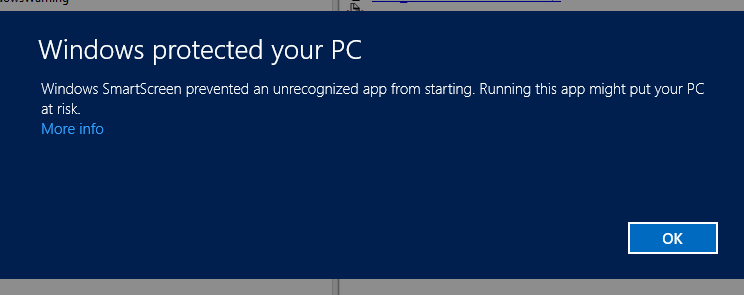
\includegraphics[scale=.5]{windowsWarning.png}
	\caption{Windows 8 warning when trying to run the installer. Select ``More Info'' and then ``Run Anyway.''}
	\label{fig:windowsWarning}
\end{figure}

When the installer file is executed, the installation will begin and show a dialog like the one shown in Figure \ref{fig:windowsInstaller}.  Users should select the default configuration, which will be the 64-bit configuration for 64-bit Windows systems, or the 32-bit configuration for 32-bit Windows systems. Click on ``Install' and the installer will install \hash on your system and then notify you when it is complete. \hash is now installed on your system can be run from the command line.\\

\begin{figure}
	\center
	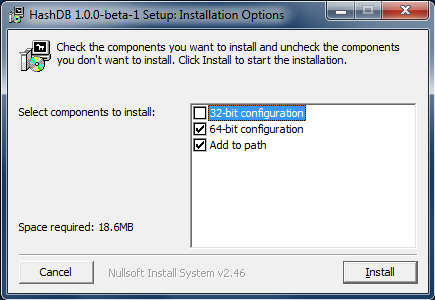
\includegraphics[scale=.8]{WindowsInstaller.png}
	\caption{Dialog appears when the user executes the Windows Installer. Select the default configuration.}
	\label{fig:windowsInstaller}
\end{figure}

\textbf{Download and Install \bulk}\\
The \bulk \hash scanner provides the capability to import block hashes into a new hash database and to scan for hashes against an existing hash database.
This scanner is included in \bulk version 1.4.5 or later. For detailed instructions on downloading and installing \bulk, please refer to the Users Manual found at \url{http://digitalcorpora.org/downloads/bulk_extractor/BEUsersManual.pdf}.

\subsection {\hash Commands}
\label{Running}
The core capabilities provided by \hash involve creating and maintaining a database of hash values and scanning media for those hash values. To perform those tasks, \hash users need to start by building a database (if an existing database is not available for use).
Users then import hashes using a DFXML file or by using the \bulk \hash scaner, and then possibly merge or subtract hashes to obtain the desired set of hashes to scan against.
Users then scan for hashes that match.
Additional commands are provided to support statistical analysis, performance tuning and performance analysis.
This section describes \hash commands, along with examples, for performing these tasks.

\subsubsection{Creating a Hash Database}
A hash database must be created before hashes can be added to it.
The command to create a hash database is shown in Table \ref{tab:createDatabase}.
To create an (empty) hash database named \textbf{\textit{mock\_video.hdb}}, type the following command:
\begin{Verbatim}[commandchars=\\\{\}]
\verbbf{hashdb create mock_video.hdb}
\end{Verbatim}
The above command will create a database with all of the default hash database settings. Most users will not need to change those settings. Our DFXML file was created with a default block size of 4096 bytes. Table \ref{tab:hashDBSettings} shows the optional parameters that can be used to specify database settings. Users can specify either the option and value or the verbose option value for each parameter along with the create command, as in:\\
\begin{Verbatim}[commandchars=\\\{\}]
\verbbf{hashdb create --max\_duplicates=20 mock_video.hdb}
\verbbf{hashdb create -m 20 mock_video.hdb}
\end{Verbatim}
The above two commands produce identical results, creating the database \textit{mock\_video.hdb} that will accept a maximum of 20 hash duplicates.\\

\begin{table}[!ht]
\centering
\caption{Commands Available in \hash Command Line Tool to Create a Database}
\label{tab:createDatabase}
\begin{tabular}{|p{2.5 cm}|p{7 cm}|p{4 cm}|}
\hline \hline
\textbf{Command} & \textbf{Usage} & \textbf{Description} \\
\hline
\textbf{create} & create [-p $<$hash block size$>$] [-m$<$maximum duplicates$>$ hashdb.hdb & Creates a new hash database with the given configuration parameters.\\
\hline
\end{tabular}
\end{table}


\begin{table}[!ht]

\centering
\caption{Settings for New Databases}
\label{tab:hashDBSettings}
\begin{tabular}{|p{1.5 cm}|p{8 cm}|p{4 cm}|}
\hline \hline
\textbf{Option} & \textbf{Verbose Option} & \textbf{Specification} \\
\hline
\textbf{\texttt{-p}} & \verb+--hash_block_size=+\textit{hash\_block\_size} & Specifies the block size (hash\_block\_size) in bytes used to generate the hashes that will be stored in the database. Default is 4096 bytes.  \\
\hline
\textbf{\texttt{-m}} & \verb+--max_duplicates=+\textit{maximum} & Specifies the maximum number of hash duplicates allowed. 0 value indicates there is no limit. Default is 0.\\
\hline
\end{tabular}
\end{table}

\subsubsection{Importing and Exporting between a DFXML File and a Hash Database}
Commands to import and export hashes are shown in Table \ref{tab:importExport}.
Once a database has been created, it may be populated with hash values from a DFXML file.
Note that there are other ways to populate a database besides importing from a DFXML file, including using other hash databases (discussed in Section \ref{updateSection}),
by using the \bulk \hash scanner (discussed in Section \ref{bulkextractorSection}),
and through the use of the import capability provided by the API (discussed in Section \ref{APISection}). \\

Using the DFXML file created in the previous section, type the following command:
\begin{Verbatim}[commandchars=\\\{\}]
\verbbf{hashdb import -r mock_video_repository mock_video.xml mock_video.hdb}
\end{Verbatim}
In the above command the option \textbf{-r} is used along with the repository name \texttt{mock\_video} \textbf{\_repository} to indicate the repository source of the block hashes being imported into the database. The repository name is used to keep track of the sources of hashes. Hash blocks contained in one database often originate from many different sources and the fileme may be the same. For example, if we add two separate but similar databases with partial overlap to a database, this will result in some duplicate hashes from multiple sources with the same filename. The repository name can be used with those duplicates to allow users to track all hashes back to their original sources. By default, the repository name used is the text \texttt{repository\_} with the filename of the file being imported from appended after it.\\


\begin{table}[!ht]
\centering
\caption{Commands Available in \hash Command Line Tool to Import and Export between DFXML Files and Hash Databases}
\label{tab:importExport}
\begin{tabular}{|p{2.5 cm}|p{7 cm}|p{4 cm}|}
\hline \hline
\textbf{Command} & \textbf{Usage} & \textbf{Description} \\
\hline
\textbf{import} & import [-r $<$ repository name $>$] $<$DFXML file.xml$>$ $<$hashdb.hdb$>$& Imports values from the DFXML file into the hash database. Command can optionally include a specific repository name to use for the set of hashes being imported\\
\hline
\textbf{export} & export $<$hashdb.hdb$>$ $<$DFXML file.xml$>$ & Exports hash database to the DFXML file\\
\hline
\end{tabular}
\end{table}


This \textbf{import} command in the above example imports the contents of \texttt{mock\_video.xml} into the database \textit{mock\_video.hdb}. \hash prints the following to the command line to indicate that the hashes have been inserted into the database successfully: 

\begingroup
\footnotesize
\begin{Verbatim}[fontfamily=courier]
hashdb changes (insert):
    hashes inserted: 2595
\end{Verbatim}
\endgroup
The database \textit{\textbf{mock\_video.hdb}} now holds 2595 hash values. Navigate into the directory, \textit{mock\_video.hdb}. It will contain a set of database files, the following lists the contents:
\begingroup
\footnotesize
\begin{Verbatim}[fontfamily=courier]
 4097 Mar  9 21:52 Bloom_filter_1
90112 Mar  9 21:56 hash_store
 3788 Mar  9 21:52 history.xml
 3573 Mar  9 21:56 log.xml
 3105 Mar  9 21:52 settings.xml
   47 Mar  9 22:21 source_filename_store.dat
 8192 Mar  9 21:56 source_filename_store.idx1
 8192 Mar  9 21:56 source_filename_store.idx2
   25 Mar  9 22:21 source_lookup_store.dat
 8192 Mar  9 21:56 source_lookup_store.idx1
 8192 Mar  9 21:56 source_lookup_store.idx2
   37 Mar  9 22:21 source_repository_name_store.dat
 8192 Mar  9 21:56 source_repository_name_store.idx1
 8192 Mar  9 21:56 source_repository_name_store.idx2
\end{Verbatim}
\endgroup

The file \texttt{log.xml} will show that a set of hash blocks have just been inserted. Listing \ref{logexcerpt} shows the excerpt of the log file that tracks this statistic.
\lstset{style=customfile}
\begin{lstlisting}[float, caption=Excerpt of the \texttt{log.xml} indicating hash blocks were inserted, label=logexcerpt]
...   
   <repository_name>repository_mock_video.xml</repository_name>
    <timestamp name='begin import' delta='0.024016' total='0.024016'/>
    <timestamp name='end import' delta='0.015009' total='0.039025'/>
    <hashdb_changes>
      <hashes_inserted>2595</hashes_inserted>      
    </hashdb_changes>
...
\end{lstlisting}
Users can also run the following command to get information about the contents of the database (and confirm that values were inserted):
\begin{Verbatim}[commandchars=\\\{\}]
\verbbf{hashdb statistics mock_video.hdb}
\end{Verbatim}

\subsubsection{Manipulating Hash Databases}
Databases may need to be merged together or common hash values may need to be subtracted out in order for them to be more suitable for scanning against.
Commands that manipulate hash databases are outlined in Table \ref{tab:databaseManipulation}.

\begin{table}[!ht]
\centering
\caption{Commands Available in \hash Command Line Tool to Manipulate Hash Databases}
\label{tab:databaseManipulation}
\begin{tabular}{|p{3.5 cm}|p{6 cm}|p{4 cm}|}
\hline \hline
\textbf{Command} & \textbf{Usage} & \textbf{Description} \\
\hline
\textbf{add} & add $<$source db$>$ $<$destination db$>$ & Copies all of the hashes from \textit{source db} to \textit{destination db}\\
\hline
\textbf{add\_multiple} &  add\_multiple $<$source db1$>$ $<$source db2$>$ $<$destination db$>$ & Performs the union of \textit{source db1} and \textit{source db2} and copies all of the hash values from the union into \textit{destination db}\\
\hline
\textbf{import} & import [-r $<$ repository name $>$] $<$DFXML file$>$ $<$hashdb$>$& Imports values from the DFXML file into the hash database. Command can optionally include a specific repository name to use for the set of hashes being imported\\
\hline
\textbf{intersect} & intersect $<$source db1$>$ $<$source db2$>$ $<$destination db$>$&   Copies hash values common to both \textit{source db1} and \textit{source db2} into \textit{destination db}\\
\hline
\textbf{subtract} & subtract $<$source db1$>$ $<$source db2$>$ $<$destination db$>$&   Copies hash values found in \textit{source db1} but not in \textit{source db2} into \textit{destination db}\\
\hline
\textbf{deduplicate} & deduplicate $<$source db$>$ $<$destination db$>$&   Copies all non-duplicate hash values from \textit{source db1} into \textit{destination db}\\
\hline
\end{tabular}
\end{table}

\subsubsection{Tracking Changes in Hash Databases}
Statistics about hash database changes are reported on the console and to the log file and history file inside the hash database.
These statistics show the number of hashes inserted or removed as a result of a command, and also show the number of hashes not inserted or not removed because specific conditions were not met.
These statistics are shown in Table \ref{tab:changeStatistics}.
\begin{table}[!ht]

\centering
\caption{Database Statistics reported on the console and tracked in the file \texttt{log.xml}}
\label{tab:changeStatistics}
\begin{tabular}{|p{5 cm}|p{8.8 cm}|}
\hline \hline
\textbf{Statistic} & \textbf{Meaning} \\
\hline
{hashes\_inserted} &  Number of hashes inserted.\\
\hline
hashes\_not\_inserted\_ mismatched\_hash\_block\_size & Number of hashes not inserted
because the hash block size of the block requested for insert was
incorrect. For example if the database requires a hash block size of 4096,
and the file size is 5096 bytes, the last block hash size will be an (invalid) 100 bytes,
so it will not be inserted. NOTE: this will occur almost every time hash blocks are added to the database since the remaining bytes of every file are not likely to be comprised of the exact hash size. This is not an error.\\
\hline
hashes\_not\_inserted\_ invalid\_byte\_alignment &  Number of hashes not inserted because the file offset was not byte aligned.
If the database expects a byte alignment of 512 and the \hash user
tries to add a hash at byte 80, \hash will detect that 80 does not fall on
a 512 byte boundary $(80 \% 512 \ne 0)$.\\
\hline
hashes\_not\_inserted\_exceeds \_max\_duplicates & Number of hashes not inserted because they exceed the max duplicates value. For example, user sets max duplicates with \texttt{-m 20} and the run attempts to import 30 hashdigests calculated from 30 NULL blocks of input, so we see 20 max duplicates.\\
\hline
hashes\_not\_inserted\_ duplicate\_element& Number of hashes not inserted because they are duplicate elements. The user attempts to import a hash where the hash value, repository name, filename, and its file offset
are all the same.\\
\hline
hashes\_removed& Number of hashes removed \\
\hline
hashes\_not\_removed\_ mismatched\_hash\_block\_size& Number of hashes not removed because the hash block size of the block requested for removal did not match the hash block size the database was configured to accept.
\\
\hline
hashes\_not\_removed\_ invalid\_byte\_alignment &  Number of hashes not removed because the file offset was not byte aligned.\\
\hline
hashes\_not\_removed\_no\_ hash&  Number of hashes not removed because the hash blocks requested for removal did not exist in the database.\\
\hline
hashes\_not\_removed\_no\_ element&  Number of hashes not removed because the hashes, specifically identified by 
hash value, repository name, filename, and its file offset do not exist in the database, indicating a possible mistake in database management.\\
\hline
\end{tabular}
\end{table}


\subsubsection{Scanning Media for Hash Values}
\hash can be used to determine if a file, directory or disk image has content that matches another file, directory or disk image. This capability can be used, for example, to determine if a set of files contains a specific file excerpt or if a media image contains a video fragment. Forensic investigators can use this feature to search for blacklisted content. To scan media for hash values, run using the \bulk \textit{hashdb} scanner on a media image file and provide a hash database created by \hash as input.
Scan services are shown in Table \ref{tab:scanServices}. \\

\begin{table}[!ht]
\centering
\caption{Commands Available in \hash Command Line Tool to Query a Database}
\label{tab:scanServices}
\begin{tabular}{|p{3.5 cm}|p{6 cm}|p{4 cm}|}
\hline \hline
\textbf{Command} & \textbf{Usage} & \textbf{Description} \\
\hline
\textbf{scan} & scan $<$path\_or\_socket$>$ $<$DFXML file$>$ & Scans the hashdb for hashes that match hashes in the DFXML file and prints out matches.\\
\hline
\textbf{scan\_expanded} & scan $<$hashdb$>$ $<$DFXML file$>$ & Scans the hashdb for hashes that match hashes in the DFXML file and prints out the repository name, filename, and file offset for each hash that matches.\\
\hline
\textbf{expand\_identified} \textbf{\_blocks} & expand\_identified\_blocks $<$hashdb$>$ $<$identified\_blocks.txt$>$ & Prints out the repository name, filename, and file offset of each hash in the \textit{hashdb} for each hash feature in the \texttt{identified\_blocks.txt} input file.\\
\hline
\textbf{server} &  hashdb.hdb $<$port number$>$ & Starts a scan service at the given port number.\\
\hline
\end{tabular}
\end{table}

First, identify the media that you would like to scan. For this example, we download and use video file \texttt{mock\_video\_redacted\_image} available at \url{http://digitalcorpora.org/downloads/hashdb/demo}.\\ 

Second, identify the existing hash database that will be used to search for hash value matches. We'll use the database \textit{\textbf{mock\_video.hdb}} that we created in the previous section. That database contains all of the block hash values from a media image. \\

Finally, run \bulk from the command line and send the required parameters to the \textit{hashdb} scanner using the \textbf{-S} option. Run the following command: 
\begin{Verbatim}[commandchars=\\\{\}]
\verbbf{bulk_extractor -e hashdb -o outdir -S hashdb_mode=scan \\}
\textbf{        -S hashdb_path_or_socket=mock_video.hdb mock_video_redacted_image}
\end{Verbatim}
This command tells \bulk to enable the \textit{hashdb} scanner and to run it in ``scan'' mode to try to match the values found in the local database \textit{\textbf{mock\_video.hdb}}. Note: other run options using \bulk are discussed further in \ref{bulkextractorSection}.\\

Listing \ref{bulkHashScan} shows the output printed to the command line as a result of the above \bulk \hash scan command. \\

\lstset{style=customfile}
\begin{lstlisting}[float, caption=Output from \bulk \hash scan, label=bulkHashScan]

\footnotesize
\begin{Verbatim}[fontfamily=courier]
bulk_extractor version: 1.4.1
Input file: mock_video_redacted_image
Output directory: outdir1
Disk Size: 12596738
Threads: 4
All data are read; waiting for threads to finish...
Time elapsed waiting for 1 thread to finish:
     (timeout in 60 min .)
Time elapsed waiting for 1 thread to finish:
    6 sec (timeout in 59 min 54 sec.)
Thread 0: Processing 0

All Threads Finished!
Producer time spent waiting: 0 sec.
Average consumer time spent waiting: 4.69167 sec.
Phase 2. Shutting down scanners
Phase 3. Creating Histograms
   ccn histogram...   ccn_track2 histogram...   domain histogram...
   email histogram...   ether histogram...   find histogram...
   ip histogram...   telephone histogram...   url histogram...
   url microsoft-live...   url services...   url facebook-address...
   url facebook-id...   url searches...
Elapsed time: 6.33812 sec.
Total MB processed: 125
Overall performance: 1.98746 MBytes/sec (0.496864 MBytes/sec/thread)
Total email features found: 0
\end{Verbatim}
\end{lstlisting}

All hash block matches discovered in the hash database are printed to the \bulk output file \texttt{identified\_blocks.txt}. Listing \ref{identifiedBlocks} shows the contents of that file after the \bulk run. Each line of the file corresponds to one hash block from the input data provided that was matched in the database. The number at the beginning of the line is the Forensic Path.\\

The \bulk program introduced the concept of the ``forensic path''. The forensic path is a description of the origination of a piece of data. It might come from, for example, a flat file, a data stream, or a decompression of some type of data. Consider an HTTP stream that contains a GZIP-compressed email as shown in Figure ~\ref{fig:forensicPath}. A series of \bulk scanners will first find the ZLIB compressed regions in the HTTP stream that contain the email, decompress them, and then find the features in that email which may include email addresses, names and phone numbers. Using this method, \bulk can find email addresses in compressed data. The forensic path for the email addresses found indicate that it originated in an email, that was GZIP compressed and found in an HTTP stream. The forensic path of the email addresses features found might be represented as shown in the example feature file in Listing \ref{forensicPathExcerpt}. It is worth nothing that the \textit{hashdb} scanner can recognize a matching block embedded in part of another file. No other existing digital forensic tool can do this; other tools find only completely unembedded files.\\
\lstset{style=customfile}
\begin{lstlisting}[float, caption=Forensic Path of email address features found in \bulk, label=forensicPathExcerpt]
11052168704-GZIP-3437  live.com  eMn='domexuser@live.com';var  srf_sDispM
11052168704-GZIP-3475  live.com  pMn='domexuser@live.com';var  srf_sDreCk
11052168704-GZIP-3512  live.com  eCk='domexuser@live.com';var  srf_sFT='<
\end{lstlisting}


\begin{figure}
	\center
	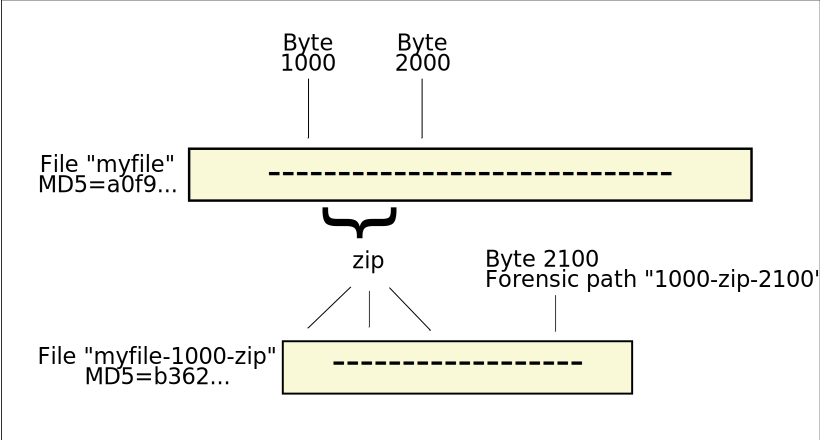
\includegraphics[scale=.55]{drawings/forensic_path}
	\caption{Forensic path of features found in email lead back to HTTP Stream}
	\label{fig:forensicPath}
\end{figure}

The second column of the \texttt{identified\_blocks.txt} file shows the actual block hash value. The final column is the number of times this block hash value has been added to the hash database. It is a count of hash duplicates. Hash duplicates occur when the hash value is the same but any part of the source information including repository name, filename or offset, is unique. In this case, each hash values shown has only been added to the database once.\\

To identify the source information associated with the hash values found in \texttt{identified\_blocks.txt}, type the following command using the hash database and \texttt{identified\_blocks.txt} file as input (command should be run from the same directory in which you ran \bulk):
\begin{Verbatim}[commandchars=\\\{\}]
\verbbf{hashdb expand_identified_blocks mock_video.hdb outdir/identified_blocks.txt} 
\textbf{  > identified_sources.txt}
\end{Verbatim}
The above command pipes the output directly into the file \texttt{identified\_sources.txt}. Each line of the file will provide the source information for one of the identified hash blocks. An example line from this file is shown in Listing \ref{identifiedSourceLine},
which shows that the block at Forensic path 12464640 matches the block 10498048 bytes into the \texttt{mock\_video.mp4} files in the hash database, indicating a positive match.\\

\lstset{style=customfile}
\begin{lstlisting}[float, caption={The \texttt{identified\_blocks.txt} file produced by \bulk's \textit{hashdb} scanner. First column is the forensic path, second is the hash value, and third is the number of times the hash value occurs in the database}, label=identifiedBlocks]
# BANNER FILE NOT PROVIDED (-b option)
# BULK_EXTRACTOR-Version: 1.4.1 ($Rev: 10844 $)
# Feature-Recorder: identified_blocks
# Filename: mock_video_redacted_image
# Feature-File-Version: 1.1
12452352	3b6b477d391f73f67c1c01e2141dbb17	1
12456448	89a170b6b9a948d21d1d6ee1e7cdc467	1
12460544	f58a09656658c6b41e244b4a6091592c	1
12464640	1d0abbddf1344ac751d17604bdd9ebe8	1
12468736	16d75027533b0a5ab900089a244384a0	1
12472832	97068927ff7ca0c4d27ac527474065bc	1
12476928	80a403ea48854676501a02e390a69699	1
12481024	7de953ea563c4df1f8369d8dd2cfb4d9	1
12485120	1b803bd6e014d1855e6f8413041c2b07	1
12489216	cf49adf3285b983d9f8d60497290bfd2	1
12493312	4cc415709e205ac0ef5b5dcfb77936b6	1
12497408	0c5c611edc8dfd34f85c6cbf88702e51	1
12501504	4a93e65fb187d71c2b8b5697f1460e3d	1
12505600	a667f79e6446222092257af1780f6a9f	1
12509696	aec94ab99f591f507b3c27424a0b52c5	1
12513792	c6361fe0eb4f7b13bac6529e1cdd8ea4	1
\end{lstlisting}

\begin{lstlisting}[float, caption={The \texttt{identified\_sources.txt} file produced by post-processing the \texttt{identified\_blocks.txt} file. First column is the forensic path, second is the hash value, and third is the repository name, filename, and file offset}, label=identifiedSourceLine]
12464640 1d0abbddf1344ac751d17604bdd9ebe8 repository name=repository_demo_
video.xml,filename=C:\md5deep\md5deep-4.3\mock_video.mp4,file offset=104
98048
\end{lstlisting}

Users may be put off by the quantity of matches incurred by low-entropy data in their databases such as blocks of zeros or metadata header blocks from files that are otherwise unique. For now, \hash provides commands for this:
\begin{itemize}
\item Use the ``subtract'' command to remove known whitelist data created from sources such as ``brand new'' operating system images and the NSRL.
\item Alternatively, use the ``deduplicate'' command to remove all hash values that have been imported more than once.
\end{itemize}
These commands are provided to manage false positives.

\subsubsection{Statistics}
Various metadata statistics are available about a given hash database including the size of a database, where its hashes were sourced from, a histogram of its hashes, and more.
Table \ref{tab:statistics} describes available statistics.

\begin{table}[!ht]
\centering
\caption{Commands Available in \hash Command Line Tool to obtain Metadata Statistics about a Hash Database}
\label{tab:statistics}
\begin{tabular}{|p{3.5 cm}|p{6 cm}|p{4 cm}|}
\hline \hline
\textbf{Command} & \textbf{Usage} & \textbf{Description} \\
\hline
\textbf{size} &  size $<$hashdb$>$ & Prints out size information relating to the database.\\
\hline
\textbf{sources} &  source $<$hashdb$>$ & Provides a top-level view of the repository names and filenames in the database. It prints out all repositories and files that have contributed to this database.\\
\hline
\textbf{histogram} & histogram $<$hashdb$>$ &  Prints a hash distribution for the hashes in the \textit{hashdb}.\\
\hline
\textbf{duplicates} & duplicates $<$hashdb$>$ $<$number$>$ &  Prints out hashes in the database that are sourced the given number of times.\\
\hline
\textbf{hash\_table} & hash\_table $<$hashdb$>$ &  Prints out a table of hashes in the database, indicating the repository name, filename, and file offset of where each hash was sourced.\\
\hline
\end{tabular}
\end{table}

\subsubsection{Tuning}
The Bloom filter may be tuned, see Table \ref{tab:tuning}.

\begin{table}[!ht]
\centering
\caption{Commands Available in \hash Command Line Tool to obtain Metadata Statistics about a Hash Database}
\label{tab:tuning}
\begin{tabular}{|p{3.5 cm}|p{6 cm}|p{4 cm}|}
\hline \hline
\textbf{Command} & \textbf{Usage} & \textbf{Description} \\
\hline
\textbf{tuning} &  tuning $<$bloom filter settings$>$ & Tunes the Bloom filter for the database.\\
\hline
\end{tabular}
\end{table}

\subsubsection{Performance Analysis}
Performance analysis commands for analyzing \hash performance are available, see Table \ref{tab:analysis}.

\begin{table}[!ht]
\centering
\caption{Commands Available in \hash Command Line Tool to perform \hash Performance Analysis}
\label{tab:analysis}
\begin{tabular}{|p{3.5 cm}|p{6 cm}|p{4 cm}|}
\hline \hline
\textbf{Command} & \textbf{Usage} & \textbf{Description} \\
\hline
\textbf{add\_random} & add\_random -r [$<$repository name$>$] $<$hashdb.hdb$>$ $<$count$>$ & Adds count random hashes to the given database, creating timing data in the \texttt{log.xml} file.\\
\hline
\textbf{scan\_random} & scan\_random $<$hashdb.hdb$>$ $<$hashdb copy.hdb$>$ & Scans the given database, creating timing data in the \texttt{log.xml} file.\\
\hline
\end{tabular}
\end{table}

\subsection{Importing and Scanning Using the \bulk \hash Scanner}
The \bulk \hash scanner may be used to import hashes and to scan for hashes.
The syntax for this scanner is shown in Table \ref{tab:hashdbScanner}.

\begin{table}[!ht]
\centering
\caption{\bulk \hash Scanner Commands}
\label{tab:hashdbScanner}
\begin{tabular}{|p{3.5 cm}|p{6 cm}|p{4 cm}|}
\hline \hline
\textbf{Command} & \textbf{Usage} & \textbf{Description} \\
\hline
\textbf{import} & bulk\_extractor -e hashdb -S hashdb\_mode=import -o outdir1 my\_image1 & Import \\
\hline
\textbf{scan} & bulk\_extractor -e hashdb -S hashdb\_mode=scan -S hashdb\_scan\_path\_or\_socket=outdir/hashdb.hdb -o outdir2 my\_image & Scan \\
\hline
\end{tabular}
\end{table}


\section{Use Cases for \hash}
There are many different ways to utilize the functionality provided by the \hash tool. In this section, we highlight some of the most common uses of the system. 


\subsection{Querying for Source or Database Information}
 Users can scan a hash database directly using various querying commands. Those commands are outlined in Table \ref{tab:scanServices}.  The ``scan'' command allows users to search for hash blocks in a DFXML file that match hash blocks in a database. This can be used to determine if content from raw media matches fragments of previously encountered data contained in a database. For example, a forensic investigator may have a disk image in evidence. Using that disk image and third party tool such as \textbf{md5deep}, the investigator can generate a DFXML file of sector block hashes. The investigator can then run the ``scan'' command with the DFXML file to see if any content from the disk image matches hash blocks of known fragments of previously encountered data. The ``sources'' and ``statistics,'' commands provide information about the source of the hash blocks and statistics about the database itself.

Each hash block stored in the database is stored with three separate pieces of source information. This complete source information is provided for each source record in the hash database, including hash duplicates. The ``expand\_identified\_blocks'' command prints out this information for hashes identified in \texttt{identified\_blocks.txt} feature files. The source information includes:
\begin{itemize}
\item Repository Name:
The repository name indicates the provenance of the dataset.
It is its description information,
such as ``Company X's intellectual property files''.
The DFXML file generated by \textbf{md5deep} does not include a repository name.
To specify your own repository name when importing,
use the \texttt{-r <repository name>} option,
specifically, \texttt{import -r <repository name>}.
Otherwise, a default repository name will be generated,
consisting of the text \texttt{repository\_}
followed by the filename of the DFXML file, including its full path.
\item Filename: The file from which the block hash was sourced. Typically, hash values are sourced from files or directories of file using \textbf{md5deep} with the recursive directory ``-r'' option. If hash values are source from raw media using the \textbf{bulk\_extractor} \textit{hashdb} scanner in \texttt{import} mode, then the Forensic Path is used as the source information.
\item File Offset: the offset, in bytes, into the file where the block hash was calculated.
\end{itemize}

\subsubsection{Querying a Remote Hash Database}
\hash also provides the capability to set up a remote socket to ``scan'' an existing database. Users can set up a database on the socket and then access the ``scan'' command via that socket. To set up the scan service, users need to provide the name of the hash database and the TCP socket that will be available for clients.
For example, the following command
starts hashdb as a server service for the hash database at path \textit{my\_hashdb.hdb} at socket endpoint \texttt{tcp://*:14500}:
 \begin{Verbatim}[commandchars=\\\{\}]
\verbbf{hashdb server my_hashdb.hdb tcp://*:14500}
\end{Verbatim} 

This example searches
the \hash server service available at socket tcp://localhost:14500 for hashes that match those in the DFXML file \texttt{my\_dfxml.xml}:
\begin{Verbatim}[commandchars=\\\{\}]
\verbbf{hashdb scan tcp://localhost:14500 my\_dfxml.xml}
\end{Verbatim} 

The only socket service \hash provides is for scanning. The \hash ``scan'' command, the \hash library API constructor for scanning and the \bulk \textit{hashdb} scanner in scan mode all accept a path or a socket and are the only place where sockets are used.\\

A note of caution, when a socket server service is opened, its associated hash databased is opened. Do not make changes to a database when it is opened as a socket server service. Although this will not corrupt the hash database, it is likely to cause the server service to perform incorrectly.\\

It is likely that the TCP port number you choose to use will need to be enabled by your firewall on the Server side.\\

There is no security in the current protocol. It should only be used on a private network.

\subsection{Writing Software that works with \hash}
\label{APISection}
\hash provides an API that other software programs can use to access two important database capabilities. The file \texttt{hashdb.hpp} found in the \textit{src} directory contains the complete specification of the API. That complete file is also contained in Appendix \ref{hashdbapi} of this document.  The two key features provided by the API include the ability to import values into a hash database and the ability to scan media for any values matching those in a given hash database.  The \bulk program uses the \hash API to implement both of these capabilities.  The following section provides more information on how to access these features. \\

\subsection{Scanning or Importing to a Database Using \bulk}
\label{bulkextractorSection}
The \bulk \textit{hashdb} scanner allows users to query for fragments of previously encountered hash values and populate a hash database with hash values. Options that control the \textit{hashdb} scanner are provided to \bulk using the ``-S name=value'' command line parameters. When \bulk executes, the parameters are sent directly to the scanner. Options include
\begin{itemize}
\item hashdb\_mode - the mode for the scanner. One of [none|import|scan] - ``none'' the scanner is active but performs no action, ``import'' - the scanner imports block hashes, ``scan'' - the scanner scans for matching block hashes
\item hashdb\_block\_size - Block size, in bytes, used to generate hashes. The default is 4096.
\item hashdb\_ignore\_empty\_blocks - Selects to ignore empty blocks.  One of [YES|NO].  The default is YES.
\item hashdb\_scan\_path\_or\_socket - The file path to a hash database or
    socket to a hashdb server to scan against.  Valid only in scan mode. No default provided. Value must be specified if in scan mode.
\item hashdb\_scan\_sector\_size - Selects the scan sector size.  Scans along sector boundaries.
      Valid only in scan mode. Default value is 512.
\item hashdb\_import\_sector\_size - Selects the import sector size.  Imports along sector boundaries.
      Valid only in import mode. Default value is 4096.
\item hashdb\_import\_repository\_name - Selects the repository name to attribute the import to.
      Valid only in import mode. Default value is ``default\_repository''.
\item hashdb\_import\_max\_duplicates - The maximum number of duplicates to import
    for a given hash value.  Valid only in import mode. The default is 0 for no limit.
\end{itemize}

For example, the following command runs the \bulk \textit{hashdb} scanner in import mode and adds hash values calculated from the disk image \texttt{my\_image} to a hash database:
\begin{Verbatim}[commandchars=\\\{\}]
\verbbf{bulk_extractor -e hashdb -o outputDir -S hashdb_mode=import my_image}
\end{Verbatim}
Note, \bulk will place feature file and other output not relevant to the \hash application in the ``outputDir'' directory. When using the import command, the output directory will contain a newly created hash database called \textit{hashdb.hdb}. That database can then be copied or added to a hash database in another location.


\subsection{Updating Hash Databases}
\label{updateSection}
\hash provides users with the ability to manipulate the contents of hash databases. The specific command line options for performing these functions are described in Table \ref{tab:databaseManipulation}. \hash databases are treated as sets with the add, subtract and intersect commands basically using add, subtract and intersect set operations. For each of the commands, the databases described in the arguments must be existing databases. For example, the following command will  copy all non-duplicate values from \textit{mock\_video.hdb} into \textit{mock\_video\_dedup.hdb} :
\begin{Verbatim}[commandchars=\\\{\}]
\verbbf{hashdb deduplicate mock_video.hdb mock_video_dedup.hdb}
\end{Verbatim}
Whenever a database is created or updated, \hash updates the file \texttt{log.xml}, found in the database's directory with information about the actions performed.\\

After each command to change a database, statistics about the changes are writen in the \texttt{log.xml} file and to \texttt{stdout}. Table \ref{tab:changeStatistics} shows all of the statistics tracked in the log file along with their meaning. The value of each statistic is the number of times the event happened during the command. For example, if 280 hashes are removed, the statistic ``hashes\_removed'' will be marked with a value of 280. \\

\subsubsection{Update Commands and ``Duplicate'' Hashes}
Commands that add or import hashes of the same value will result in hash duplicates if the source information is unique. If hash and source values are identical (including repository name), no hash values are added with the \textbf{add} or \textbf{import} commands. The \textbf{intersect} and \textbf{subtract} commands do not require source information to match. An intersection occurs when hatches match, regardless of whether the source information matches. Similarly, hash values are also subtracted from the database regardless of whether or not their source information matches.  The update statistics specified in the log file (shown in \ref{tab:changeStatistics}) will specify the results of each of these commands to help users track changes. \\

As discussed previously, users can only specify the repository name with the \textbf{import} command. As databases become large, the repository name for each hash value will help identify important source information. Users should plan on importing data with specific repository names whenever possible to avoid source confusion later.\\

Finally, we provide two philosophies for mitigating duplicate hash bloat:
\begin{itemize}
 \item If you know you have imported the same blacklist data twice,
  and you do not want to manage a 'whitelist' database,
  \texttt{deduplicate} is a quick and easy way to get rid of low-entropy noise.
  \item If your database has blacklist data from more than one source
  or you just want tighter control about what you want to remove
  and are willing to use a 'whitelist' database
  to remove hashes to improve lookup speed
  or to reduce noise about uninteresting hashes found,
  use \texttt{subtract}.
\end{itemize}







\subsection{Optimizing a Hash Database}
\label{optimizing}
 
For large databases, it takes a bit of time to look up a hash value to determine whether it is in the database. This time adds up when scanning for millions of hash values. As an optimization, \hash provides the capability to utilize a Bloom filter to speed up performance during hash queries. A Bloom filter is a data structure that is used to determine if a member is not part of a set. In \hash, a Bloom filter can be used to quickly indicate if a hash value is not part of the database. If the Bloom filter indicates a hash value is definitely not in the hash database, no actual hash database look up is necessary. If the Bloom filter says the hash value may be in the database, a look up is still required and no time is saved. The disadvantage of using a Bloom filter is that it can consume large amounts of disk space and memory. A Bloom filter that is too small fills up and then too often gives false positives that indicate the hash value might be in the database. A Bloom filter that is too large will take up too much memory and disk space.\\

\hash has a Bloom filter.  Users can enable or disable this Bloom filter and tune it using information about the hashes and hash functions. The optimal configuration for the Bloom filter depends on the size of the dataset. Although several tuning controls are available, we recommend only using ``bloom1\_n $<$n$>$,'' where ``n'' is the expected number of hashes in the dataset. If users want to improve scan speed, they should tune Bloom 1 based on their database size using this option. The default setting for the Bloom filter in \hash is enabled, is tuned for about 45,000,000 hashes, and takes up about 33MB of space. 

\subsection{Exporting Hash Databases}
Users can export hashes from a hash database to a DFXML file using the ``export'' command. For example, the following command will export the \textit{mock\_video.hdb} database to the file \texttt{demoVideoHashes.xml}:
\begin{Verbatim}[commandchars=\\\{\}]
\verbbf{hashdb export mock_video.hdb demoVideoHashes.xml}
\end{Verbatim}

Note that the DFXML that \hash exports is compatible but different from the DFXML created by \texttt{md5deep}. Listing \ref{dfxmlHashExport} shows an example excerpt of a DFXML file exported from \hash. The differences are:
\begin{enumerate}
\item The first offset is 6938624, not 0,
because the output is sorted by hash value. 
\item There is a \texttt{fileobject} tag wrapping every individual hash.
\item Every entry includes a \texttt{repository\_name} tag.
\end{enumerate}

\lstset{style=customfile}
\begin{lstlisting}[float, caption=Excerpt of a DFXML exported by \hash, label=dfxmlHashExport]
  <fileobject>
    <repository_name>repository_mock_video.xml</repository_name>
    <filename>/home/bdallen/demo/mock_video.mp4</filename>
    <byte_run file_offset='6938624' len='4096'>
      <hashdigest type='MD5'>0016aa775765eb7929ec06dea25b6f0e</hashdigest>
    </byte_run>
  </fileobject>
  <fileobject>
    <repository_name>repository_mock_video.xml</repository_name>
    <filename>/home/bdallen/demo/mock_video.mp4</filename>
    <byte_run file_offset='3837952' len='4096'>
      <hashdigest type='MD5'>00183a37c80b3ee02cb4bdd3e7d7e9d2</hashdigest>
    </byte_run>
  </fileobject>\
  <fileobject>
    <repository_name>repository_mock_video.xml</repository_name>
    <filename>/home/bdallen/demo/mock_video.mp4</filename>
    <byte_run file_offset='5652480' len='4096'>
      <hashdigest type='MD5'>00513c9484ebc957eb928adf30504bc9</hashdigest>
    </byte_run>
  </fileobject>
\end{lstlisting}


\section{Worked Example: Finding Similarity Between Disk Images}
The worked example provided is intended to further illustrate how to use \hash to answer specific questions and perform specific tasks.  This example uses a publicly available dataset and can be replicated by readers of this manual.  In this example, we walk through the process of using \hash (and \bulk) to find the similarities between two separate disk images. We generate a hash database of block hashes from each media image and then obtain common block hashes by taking the intersection of the two databases.\\

First, we download two files to use for comparison. The disk images are called \texttt{jo-favorites} \texttt{-usb-2009-12-11.E01} and \texttt{jo-work-usb-2009-12-11.E01}. Both files are available at \url{http://digitalcorpora.org/corp/nps/scenarios/2009-m57-patents/drives-redacted/}. Specifically with this example, we will be comparing the contents of two fictional USB drives.\\

Then, we run \bulk on each disk image separately:
\begin{Verbatim}[commandchars=\\\{\}]
\verbbf{bulk_extractor -o workOutput -S hashdb_mode=import  jo-work-usb-2009-12-11.E01}
\end{Verbatim}

\bulk writes the following output to the screen, indicating a successful run:
\begingroup
\footnotesize
\begin{Verbatim}[fontfamily=courier]
bulk_extractor version: 1.4.1
Input file: jo-work-usb-2009-12-11.E01
Output directory: workOutput
Disk Size: 131072000
Threads: 1
21:57:21 Offset 67MB (51.20%) Done in  0:00:24 at 21:57:45
All data are read; waiting for threads to finish...
Time elapsed waiting for 1 thread to finish:
    1 sec (timeout in 59 min 59 sec.)
All Threads Finished!
Producer time spent waiting: 38.5587 sec.
Average consumer time spent waiting: 1.85768 sec.
*******************************************
** bulk_extractor is probably CPU bound. **
**    Run on a computer with more cores  **
**      to get better performance.       **
*******************************************
Phase 2. Shutting down scanners
Phase 3. Creating Histograms
   ccn histogram...   ccn_track2 histogram...   domain histogram...
   email histogram...   ether histogram...   find histogram...
   ip histogram...   telephone histogram...   url histogram...
   url microsoft-live...   url services...   url facebook-address...
   url facebook-id...   url searches...
Elapsed time: 47.6743 sec.
Total MB processed: 1310
Overall performance: 2.74932 MBytes/sec (2.74932 MBytes/sec/thread)
Total email features found: 31
\end{Verbatim}
\endgroup


Next, run \bulk on the other usb drive disk image:
\begin{Verbatim}[commandchars=\\\{\}]
\verbbf{bulk_extractor -o favoritesOutput -S hashdb_mode=import jo-favorites-usb-2009-11.E01}
\end{Verbatim}

\bulk runs, printing the following to the screen: 
\begingroup
\footnotesize
\begin{Verbatim}[fontfamily=courier]
bulk_extractor version: 1.4.1
Input file: jo-favorites-usb-2009-12-11.E01
Output directory: favoritesOutput
Disk Size: 1048576000
Threads: 1
21:59:44 Offset 67MB (6.40%) Done in  0:05:07 at 22:04:51
22:00:08 Offset 150MB (14.40%) Done in  0:04:30 at 22:04:38
22:00:32 Offset 234MB (22.40%) Done in  0:03:59 at 22:04:31
22:00:40 Offset 318MB (30.40%) Done in  0:02:55 at 22:03:35
22:00:41 Offset 402MB (38.40%) Done in  0:02:05 at 22:02:46
22:00:42 Offset 486MB (46.40%) Done in  0:01:31 at 22:02:13
22:00:44 Offset 570MB (54.40%) Done in  0:01:07 at 22:01:51
22:00:45 Offset 654MB (62.40%) Done in  0:00:49 at 22:01:34
22:00:47 Offset 738MB (70.40%) Done in  0:00:35 at 22:01:22
22:00:48 Offset 822MB (78.40%) Done in  0:00:23 at 22:01:11
22:00:50 Offset 905MB (86.40%) Done in  0:00:13 at 22:01:03
22:00:51 Offset 989MB (94.40%) Done in  0:00:05 at 22:00:56
All data are read; waiting for threads to finish...
Time elapsed waiting for 1 thread to finish:
     (timeout in 60 min .)
All Threads Finished!
Producer time spent waiting: 76.8042 sec.
Average consumer time spent waiting: 1.79526 sec.
*******************************************
** bulk_extractor is probably CPU bound. **
**    Run on a computer with more cores  **
**      to get better performance.       **
*******************************************
Phase 2. Shutting down scanners
Phase 3. Creating Histograms
   ccn histogram...   ccn_track2 histogram...   domain histogram...
   email histogram...   ether histogram...   find histogram...
   ip histogram...   telephone histogram...   url histogram...
   url microsoft-live...   url services...   url facebook-address...
   url facebook-id...   url searches...
Elapsed time: 89.1399 sec.
Total MB processed: 10485
Overall performance: 11.7633 MBytes/sec (11.7633 MBytes/sec/thread)
Total email features found: 2
\end{Verbatim}
\endgroup

After \bulk runs, two output directories are created. Each directory contains a hash database called \textit{hashdb.hdb}. The hash databases each contain cryptographic block hashes produced from the disk images. Next, we create a database that will store the intersection of the two disk images. The following command creates the database \textit{intersection.hdb}:
\begin{Verbatim}[commandchars=\\\{\}]
\verbbf{hashdb create intersection.hdb}
\end{Verbatim}

Next, we populate the database \textit{intersection.hdb} with values that are common between the two databases using the following command:
\begin{Verbatim}[commandchars=\\\{\}]
\verbbf{hashdb intersect workOutput/hashdb.hdb favoritesOutput/hashdb.hdb intersection.hdb}
\end{Verbatim}

\hash prints the following indicating that 32 hashes were inserted successfully and 8 hashes were not inserted because they were considered to be duplicate elements (same hash and same source information):
\begingroup
\footnotesize
\begin{Verbatim}[fontfamily=courier]
hashdb changes (insert):
    hashes inserted=32
    hashes not inserted, duplicate element=8
\end{Verbatim}
\endgroup

Now, the database \textit{intersection.hdb} contains hashes common to both disk images. \\

Here are some ways to gain knowledge from the common hashes identified:
\begin{itemize}
\item Constrain the matches further by using the \texttt{intersect} command
to intersect the database with a blacklist database,
and then use the \texttt{get\_sources} command
to find the blacklist filenames that these hash values correspond to.
\item Use \bulk \textbf{Viewer} to navigate to the data that these hashes were generated from
to see if the raw data there is significant.
\item If the scanned image contains a file system,
try to use the \textbf{fiwalk} tool to carve the files from which the hash values
were calculated.
\end{itemize}



\section{Troubleshooting}
\label{DebuggingHashdb}
All \hash users should join the \bulk users Google group for more information and help with any issues encountered. To join, send an email to \textbf{bulk\_extractor-users+subscribe@} \textbf{googlegroups.com}.  \\
\section{Related Reading}
There are other articles related to block hashing, and its practical and research applications. Some of those articles are specifically cited throughout this manual. Other useful references include but are not limited to:
\begin{itemize}
\item Garfinkel, Simson, Alex Nelson, Douglas White and Vassil Rousseve. Using purpose-built functions and block hashes to enable small block and sub-file forensics. Digital Investigation. Volume 7. 2010. Page S13--S23. \url{http://www.dfrws.org/2010/proceedings/2010-302.pdf}.
\item Foster, Kristina. Using Distinct Sectors in Media Sampling and Full Media Analysis to Detect Presence of Documents From a Corpus. Naval Postgraduate School Masters Thesis, September 2012. \url{http://calhoun.nps.edu/public/handle/10945/17365}.
\end{itemize}

\bibliographystyle{acm} 
\bibliography{references}

\newpage
\appendix
\appendixpage

\section{Output of \hash Help Command}
\label{HelpOutput}
\begingroup
\footnotesize
{
\fontfamily{courier}\selectfont
\verbatiminput{hashdbUsage.txt}
}
\endgroup


\section{\hash API: \texttt{hashdb.hpp}}
\label{hashdbapi}
\lstset{language=C++}
\lstset{basicstyle=\footnotesize}
\lstset{breaklines=true}
\lstset{breakatwhitespace=true}
\lstinputlisting{hashdb.hpp}


\section{\bulk \textit{hashdb} Scanner Usage Options}
\label{scannerOptionsAppendix}
The \bulk hashdb scanner provides two capabilities: 1) scanning
a hash database for fragments of previously encountered hash values,
and 2) importing block hashes into a new hash database.
Options that control the hashdb
scanner are provided to \bulk using "-S name=value" parameters
when \bulk is invoked.  Available options are: 

\begingroup
\footnotesize
{
\fontfamily{courier}\selectfont
\verbatiminput{hashdbScannerUsage.txt}
}
\endgroup
\end{document}
